% Chapter Template

\chapter{Diseño e Implementación} % Main chapter title

\label{Chapter3} % Change X to a consecutive number; for referencing this chapter elsewhere, use \ref{ChapterX}

A continuación se describe el \textit{hardware} seleccionado para la extensión del circuito cargador, los criterios tomados en cuenta para su selección, el diseño del circuito y su conexión en \ref{sec:hard}. Luego se describe la arquitectura del sistema en \ref{sec:arq} y entra mas en detalle en \ref{sec:firm}, donde se describe el funcionamiento del \textit{firmware}. 

%----------------------------------------------------------------------------------------
%	SECTION 1
%----------------------------------------------------------------------------------------
\section{Hardware}
\label{sec:hard}

%-----------------------------------
%	SUBSECTION 1
%-----------------------------------
\subsection{El Panel Solar}
\label{subsec:panel} 
En el mercado existen distintas soluciones comerciales que se ajustan a las necesidades de cada aplicación. Ofrecen garantía limitada de entre 10 y 25 años y eficiencia de hasta 20 \% para módulos multicelda.
Es importante que los manufacturadores de módulos aseguren un control de calidad en las celdas fotovoltaicas. Estas están clasificadas según los defectos que puedan tener, identificadas con las letras A a la D. Celdas de grado A son aquellas que no presentan defectos visuales y cumplen con las especificaciones de los datos eléctricos \citep{grado}.

El sistema fotovoltaico propuesto originalmente esta basado en módulos con voltaje de 12V y 0.5A. Como medida de mitigación de riesgos, se planteó emplear componentes disponibles en el mercado local, y luego de tener en cuenta factores como grado de calidad (A), eficiencia, costos, tiempo de entrega, soporte pos-venta y al ser de Industria Argentina, se seleccionó el \textit{módulo fotovoltaico policristalino de alto rendimiento KS10T} \citep{solar} de la figura \ref{fig:ks10t} de SOLARTEC S.A.

Se trata de paneles fabricados en base a celdas de silicio policristalino de alta eficiencia. La eficiencia de estas celdas es superior al 14\%.

Cuenta con certificado IRAM (Instituto Argentino de Normalización y Certificación), certificados CE (European Union: IEC61215 \textit{Photovoltaic Solar Testing Specifications} y IEC 61730 {\textit{Photovoltaic (PV) Module Safety Qualification}) y RoHs (\textit{DIRECTIVE 2002/95/EC: Restriction of Hazardous Substances}). Éste último le agrega ventaja frente a líderes del mercado internacional que no cumplen con la restricción de determinadas sustancias peligrosas. Sus características se muestran en la tabla \ref{tab:ks10t}. 
%y figura \ref{fig:mecanicas}\footnote{Fuente: SOLARTEC S.A. Todas las distancias están expresadas en mm.}.

 \begin{figure}[h!]
	\centering
    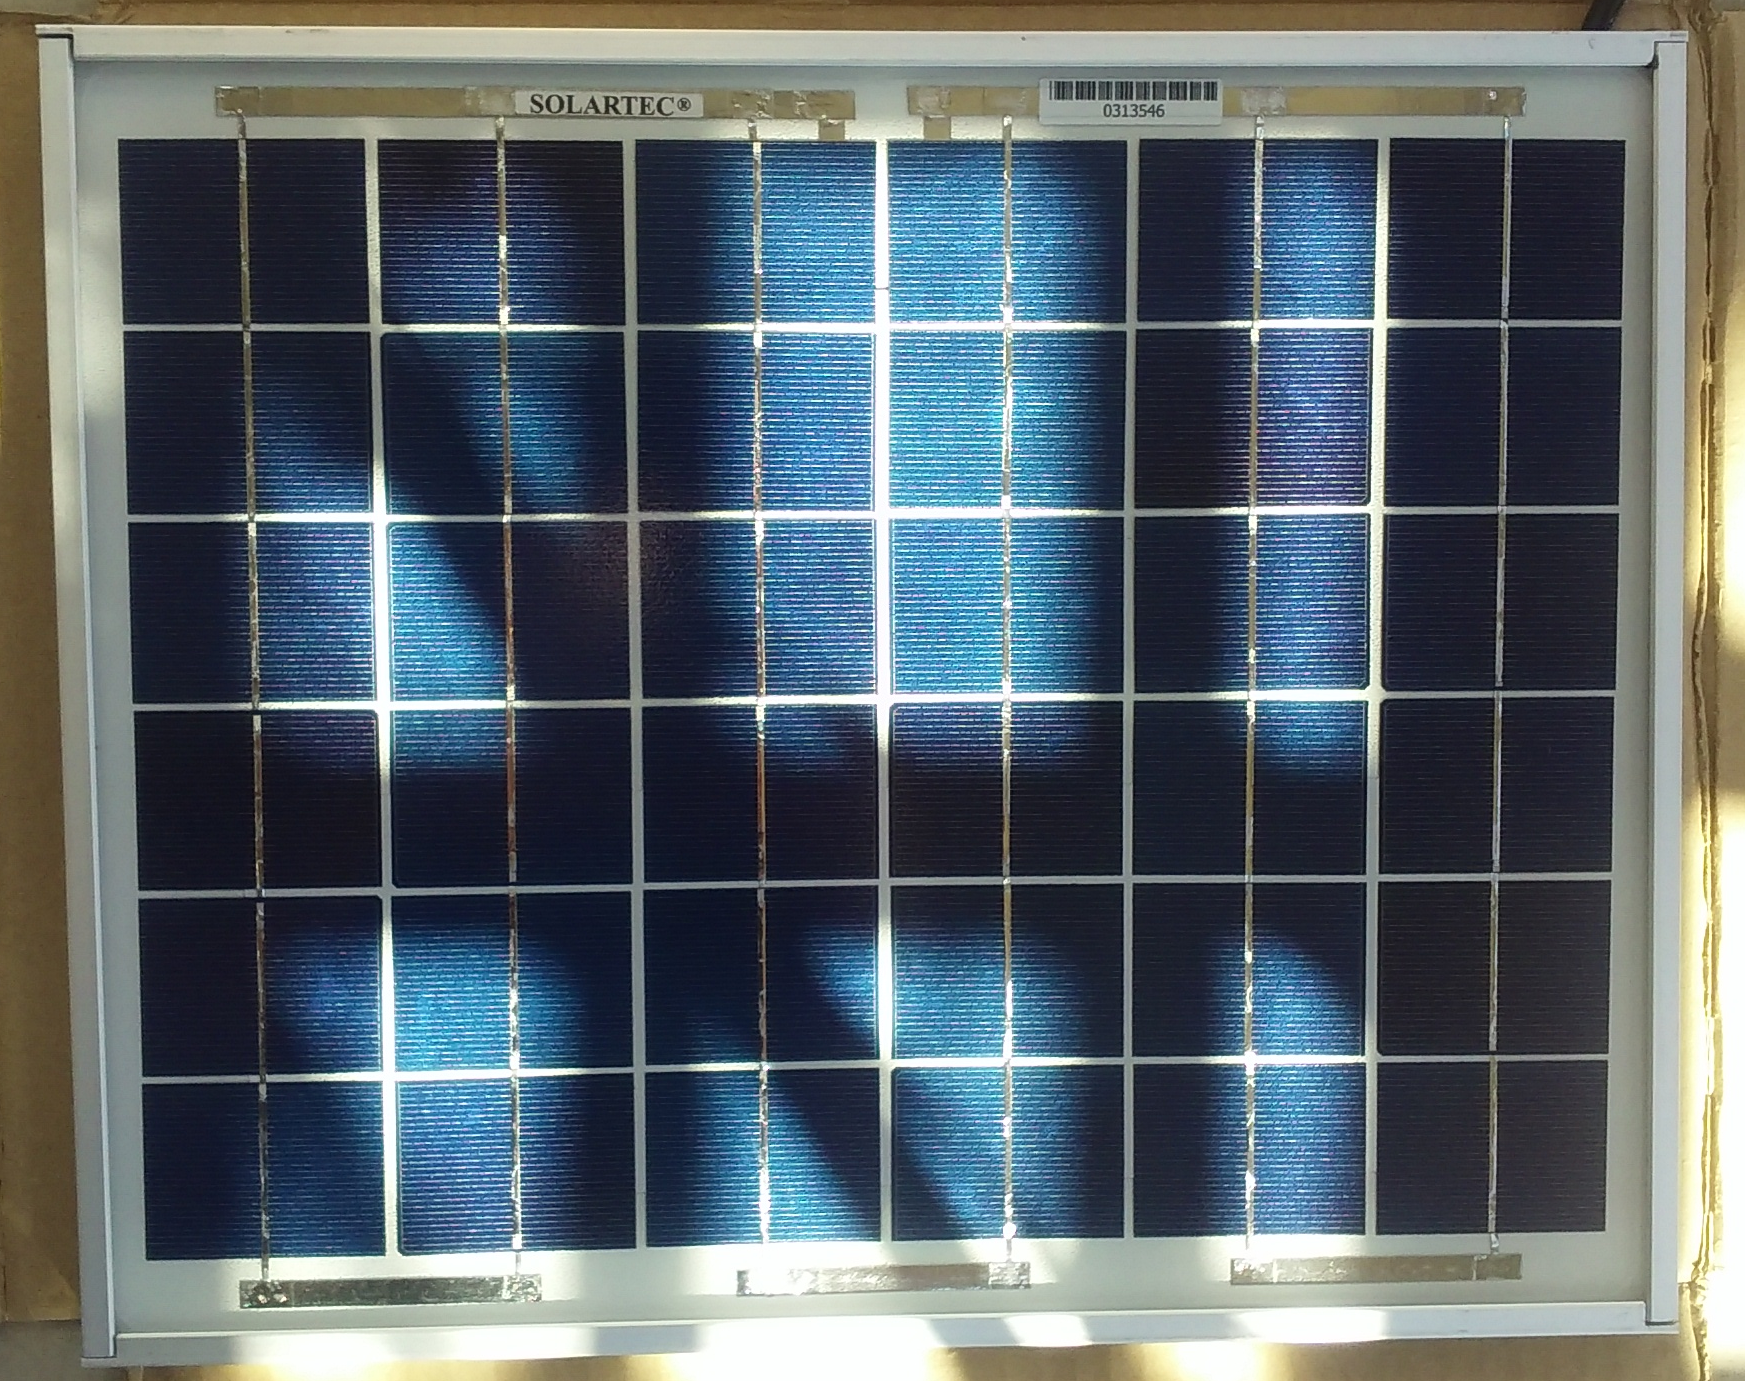
\includegraphics[width=0.6\textwidth]{./Figures/panel.png}
    	\caption{Módulo Fotovoltaico policristalino de alto rendimiento KS10T.}
	\label{fig:ks10t}
\end{figure}

\vspace{10px}

\begin{table}[ht]
	\centering
	\caption{Características del módulo fotovoltaico KS10T}
	\begin{tabular}{@{} l *2c @{}}    \toprule
		\emph{\textbf{Características}} & \emph{\textbf{Valor}} & \emph{\textbf{Unidad}}\\
		\midrule
		Potencia nominal	& 10 	& Wp	\\	
		Tensión a PN		& 17.4	& V\\
		Corriente a PN	& 0.58		& A\\
		Dimensiones		& 301x352x22 	& mm\\
		Peso				& 0.58		& Kg	\\
		\bottomrule
		\hline
	\end{tabular}
	\label{tab:ks10t}
\end{table}

La curva de la figura \ref{fig:curva}, muestra la corriente máxima de cortocircuito y la tensión máxima a circuito abierto del módulo \textit{KS10T}. Nótese que es capaz de entregar la tensión hasta exigir el máximo de corriente. Los valores y la curva están dados para condiciones de insolación de 1 KW/m2, masa atmosférica 1.5 y temperatura de celda de 25 \grados C.\footnote{Fuente: SOLARTEC S.A.}

%\begin{figure}[h]
%\centering
%\begin{subfigure}{.5\textwidth}
%%\begin{minipage}{\linewidth}
%  \centering
%    \includegraphics[width=0.5\textwidth]{./Figures/curva.JPG}
%  \caption[a)]{a)\protect\footnotemark}
%	\label{fig:curva}
%%\end{minipage}
%\end{subfigure}%
%\begin{subfigure}{.5\textwidth}
%  \centering
%    \includegraphics[width=0.5\textwidth]{./Figures/mecanicas.JPG}
%  	\caption[b)]{b)\protect\footnotemark}
%	\label{fig:mecanicas}
%\end{subfigure}
%\caption{a)Características eléctricas. b)Características mecánicas.}
%\label{fig:caract}
%\end{figure}

%\begin{figure}[h!]
%	\centering
%    \includegraphics[width=0.5\textwidth]{./Figures/mecanicas.JPG}
%    	\caption{Características mecánicas.}
%	\label{fig:mecanicas}
%\end{figure}

\begin{figure}[h!]
	\centering
    \includegraphics[width=0.6\textwidth]{./Figures/curva.JPG}
    	\caption{Características eléctricas.}
	\label{fig:curva}
\end{figure}

%-----------------------------------
%	SUBSECTION 2
%-----------------------------------
\subsection{Extensión de Circuito Cargador}
\label{subsec:extensión}
Entre las interfaces para el usuario del nodo \textit{Mote LSE} esta el puerto USB, el cual alimenta al circuito de control de carga \textit{bq24080 1-A} con 5V(DC) a través de un conector USB micro-B. Este circuito es el empleado para la carga de la batería de Li-ion de 3.7V y 900mAh.

Es por esto que es necesario emplear una etapa reguladora de voltaje a la salida del panel, para la cual se utiliza el clásico regulador de Fairchild \textit{LM7805} de 1A \citep{7805}. Que con unos pocos componentes (un condensador electrolítico como filtro a tierra para señales continuas para moderar la tensión eléctrica y las fluctuaciones de corriente y un condensador de poliéster para filtrar las señales espúreas de alta frecuencia, a la entrada y a la salida) entrega una salida de voltaje entre 4.75V y 5.25V. Además, ofrece protección contra sobrecarga térmica y cortocircuitos y opera entre -40 \grados C y +125 \grados C.

\begin{figure}[h!]
	\centering
    \includegraphics[width=1\textwidth]{./Figures/circuito.jpg}
    	\caption{Diseño de extensión de circuito cargador.}
	\label{fig:circuito}
\end{figure}

Un diseño de circuito alternativo, de montaje superficial, puede hacerse empleando el regulador \textit{TA78M05} de Toshiba Semiconductor. Ver la aplicación del circuito \textit{Current Boost Regulation} en \citep{78M05}.

%Para ver el diseño del PCB de la Extensión de Circuito Cargador, ver \ref{AppendixA}.

%-----------------------------------
%	SUBSECTION 3
%-----------------------------------
\subsection{Diagrama de conexión}
\label{subsec:conexión}

%----------------------------------------------------------------------------------------
%	SECTION 2
%----------------------------------------------------------------------------------------
\section{Arquitectura}
\label{sec:arq}
Cuando se diseña adecuadamente, los drivers del hardware están abstraídos del hardware en sí. Para que los usuarios finales, en este caso desarrolladores de software a nivel de aplicación, puedan controlar el hardware cuando una rutina en particular es llamada con el parámetro apropiado (API-CAPI \footnote{Application Programming Interface - Common Application Programming Interface}). Esto se refiere a la interfaz que las aplicaciones pueden usar para comunicarse directamente con el \textit{Mote LSE}.

Primero se usa la función del CMSIS, luego se define en código el handler de la excepción correspondiente, escribiendo en cada entrada del vector la dirección de memoria del handler asociado a la excepción.

El modelo propuesto consiste en una arquitectura de capas, a continuación se describe los niveles de abstracción desde los registros primitivos del hardware hasta la aplicación implementada (Ver subsección \ref{subsec:capas}), que incluye varios algoritmos y procedimientos (Ver subsección \ref{subsec:bloques}) que son usados para decidir de forma autónoma el modo de operación, si es necesario cargar la batería y generar alarmas de salud.

%-----------------------------------
%	SUBSECTION 1
%-----------------------------------
\subsection{Modelo de capas}
\label{subsec:capas} 
Los niveles de abstracción se describen en las siguientes capas:
cc2520.c
Implementa las funciones de acceso al transceiver cc2520
cc2520.h
contiene todas las macro que contro 

cc2520-mac.h
Define el tipo de datos necesarios para completar la trama (MHR, MAC Payload y MFR y PHR). Todos definidas en cc2520-task, mientras que el MFR (RSSI y CRC) y el SHR (secuencia de preambulo y start of frame delimiter) es implementado por hardware por el cc2520 y completa la trama. 
Especifica el tipo de trama, el modo de direccionamiento MAC (short o extended, 16 o 64 bits) y la estructura de los octetos que forman el PSDU.
cc2520-mac.c
Implementa las funciones de acceso al medio, arma el frame control field
CSMA/CA

cc2520-task.c
Esta funcion arma una trama de tipo DATA (formada con los parametros relativos al 802.15.4 de cc2520-mac.c) y la guarda en el buffer de salida. Los parametros de entrada son la direccion de destino y el payload que contiene todos las mediciones y estados de alarmas. 
y llama la funcion ccTx del cc2520-mac, que se fija en el buffer de tx si contiene un frame y lo transmite
Luego en ccTask implementa una FSM con los estados de enviar, recibir y esperar.
cc2520-task.h
Se incluyeron los estados de operacion referentes al transceiver (idle, dataRequest, waitingData, etc)
y la funcion FrameForming para ser utilizada por las capas de aplicacion superiores
se define la variable MAX RETRIES y las direcciones del coordinado, local y el PAN ID


\begin{figure}[h!]
	\centering
    \includegraphics[width=.5\textwidth]{./Figures/arq.png}
    	\caption{Modelo de Capas del Sistema.}
	\label{fig:capas}
\end{figure}
%-----------------------------------
%	SUBSECTION 2
%-----------------------------------
\subsection{Diagrama en bloques}
\label{subsec:bloques} 
Diagrama funcional.
Alarmas.
Modos.
%Módulos. 
%GPIO configurable al recibir un frame de determinadas características (puede esperar tramas de una serie de direcciones - frame filtering)

%----------------------------------------------------------------------------------------
%	SECTION 3
%----------------------------------------------------------------------------------------
\section{Firmware}
\label{sec:firm}
El software embebido, llamado firmware en adelante, fue implementado en lenguaje de programación C y assembler.

Es por una de las 6 alarmas: La temperatura de la bateria, sobre la medición de temperatura de batería, el bq24080 no es capaz de medir la temperatura de la batería (el bq24081 si). Un método para medir la temperatura de la batería sin sensores de temperatura es el método de medición basado en espectroscopia de impedancia electroquímica\citep{metodo}. Para lo cual se implementaría en el firmware una simple asignación de temperatura basada en la impedancia, pero con el bq24080 tampoco es posible medir la impedancia.

Como la hoja de datos del bq24080 y 1 estan en el mismo doc, no me habia percatado que era solo uno de los dos con el que podía medir la temp de la bateria.
Obviamente, podría agregarle sensores al Mote LSE, pero modificarlo no es parte del presente trabajo, por las implicaciones de diseño.
En rigor, esta medición en especifico no es uno de los objetivos, pero si un requerimiento de software, que se plantea para trabajo futuro.
%Algunas tareas tienen deadlines, otras pueden no tener o pueden tener poca penalidad si no se cumplen.

%#includes

%La función main siempre es llamada cuando el programa se ejecuta por primera vez. De ahi se llama a otras funciones

%-----------------------------------
%	SUBSECTION 1
%-----------------------------------
\subsection{Descripción}
\label{subsec:desc} 

Configuración de cada nodo (Tabla con Parámetros y valores)
%Master: %Configurar como MASTER %Parámetros a ingresar %Diagrama de algoritmo
%Device: %Configurar como DEVICE %Parámetros a ingresar %Diagrama de algoritmo

Para cumplir con el requerimiento de almacenar en una memoria no volátil los datos de alarma, parámetros monitoreados, tiempo total de uso, y cantidad de ciclos de carga/descarga, éstos son almacenados en la memoria Flash del microcontrolador (la memoria SRAM necesita energía para que perduren los datos). Para ello se definieron las siguientes variables:
    
%No se programan tareas con prioridades, es decir que la ejecución de una tarea no sera detenida por el procesador, sin prevaciado y no se implementa tail-chaining ni late-arriving.
%Arquitectura RISK. Modelo Hardvard: Buses separados, pero un unico mapa de memoria que esta predefinido por la arquitectura. Permite agrupar a los perifeicos por funcion y prioridad, lo que simplifica el diseno del microcontrolador y optimiza la velocidad de acceso al mismo.

Como premisa, modo sleep,
\textit{wait for interrupt} buena practica
%(_WFI)

Para ver una descripción del firmware en pseudocódigo y sus principales funciones, ver \ref{AppendixC}.

%-----------------------------------
%	SUBSECTION 2
%-----------------------------------
\subsection{Funcionalidades por capas}
\label{subsec:func} 
\begin{itemize}
	\item Implementación de funcionalidades en la subcapa PHY
	
	\item Implementación de funcionalidades en la subcapa MAC

	\item Implementación de funcionalidades a nivel de aplicación
	
\end{itemize}

%-----------------------------------
%	SUBSECTION 3
%-----------------------------------
\subsection{Ajustes a Microstack 802.15.4}
\label{subsec:stack} 
Como punto de partida, se tomo el Microstack 802.15.4 de (Ref.?) y se realizaron las siguientes modificaciones:
%-----------------------------------
%	SUBSECTION 4
%-----------------------------------
\subsection{Diagramas de Topologías Implementadas}
\label{subsec:topo} 

\begin{figure}[h!]
	\centering
    \includegraphics[width=.8\textwidth]{./Figures/topologia.jpg}
    	\caption{1) Topología estrella. 2)Topología Peer-to-Peer.}
	\label{fig:topo}
\end{figure}

\begin{figure}[h!]
	\centering
    \includegraphics[width=.8\textwidth]{./Figures/cluster.jpg}
    	\caption{Topología árbol de cluster.}
	\label{fig:clust}
\end{figure}

